%------------------------------------------------
% Incident.tex
%
% This document build the incident frame
%------------------------------------------------
\section{Incident Management}
\frame
{
\frametitle{Contenuti}
\tableofcontents[currentsection]
%\addtocounter{framenumber}{-1}
}

\subsection*{Input e Output}
\begin{frame}{Input e Output}
\begin{table}
\begin{tabular}{ l | l }
\textbf{Input} & \textbf{Da}\\
\hline
Incidente (ticket) & Utenti\\
Soluzione a problemi & Problem Management\\
Risposte a RFC & Change Management\\
\end{tabular}
\caption{Input di processo}
\end{table}
\begin{columns}
\begin{column}{0.3\textwidth}
\begin{figure}

\includegraphics[scale=0.1]{Images/Input_output.png}
\end{figure}
\end{column}
\begin{column}{0.7\textwidth}
\begin{table}
\begin{tabular}{ c | c }
\textbf{Output} & \textbf{Da}\\
\hline
Notifiche & Utenti\\
\end{tabular}
\caption{Output di processo}
\end{table}
\end{column}
\end{columns}
\end{frame}

\subsection*{Metriche di processo}
\begin{frame}{Metriche}
Saranno prodotti report mensili con le seguenti metriche:
\begin{itemize}
\item{numero totale di incidenti - suddivisi per stato - non risolti}
\item{numero e percentuale di incidenti gravi}
\item{tempo medio per la produzione di un risultato}
\item{percentuale di incidenti risolti entro SLA}
\item{numero di incidenti riaperti}
\end{itemize}
\begin{figure}
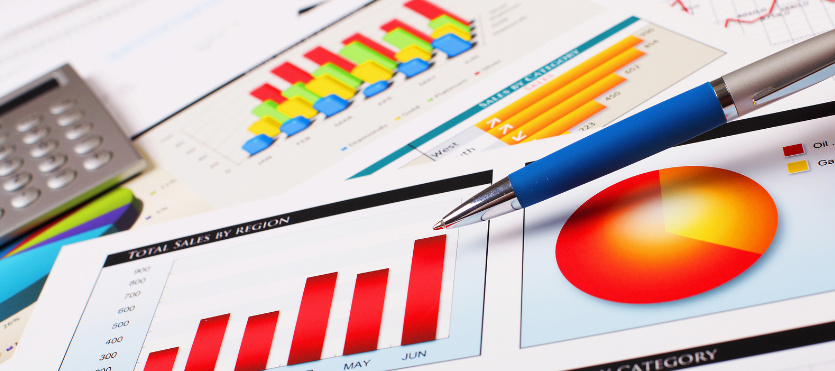
\includegraphics[scale=0.13]{Images/Metrics.png}
\end{figure}
\end{frame}

\subsection*{Attività di processo}
\begin{frame}{Attività di processo \small{1/2}}
\begin{figure}
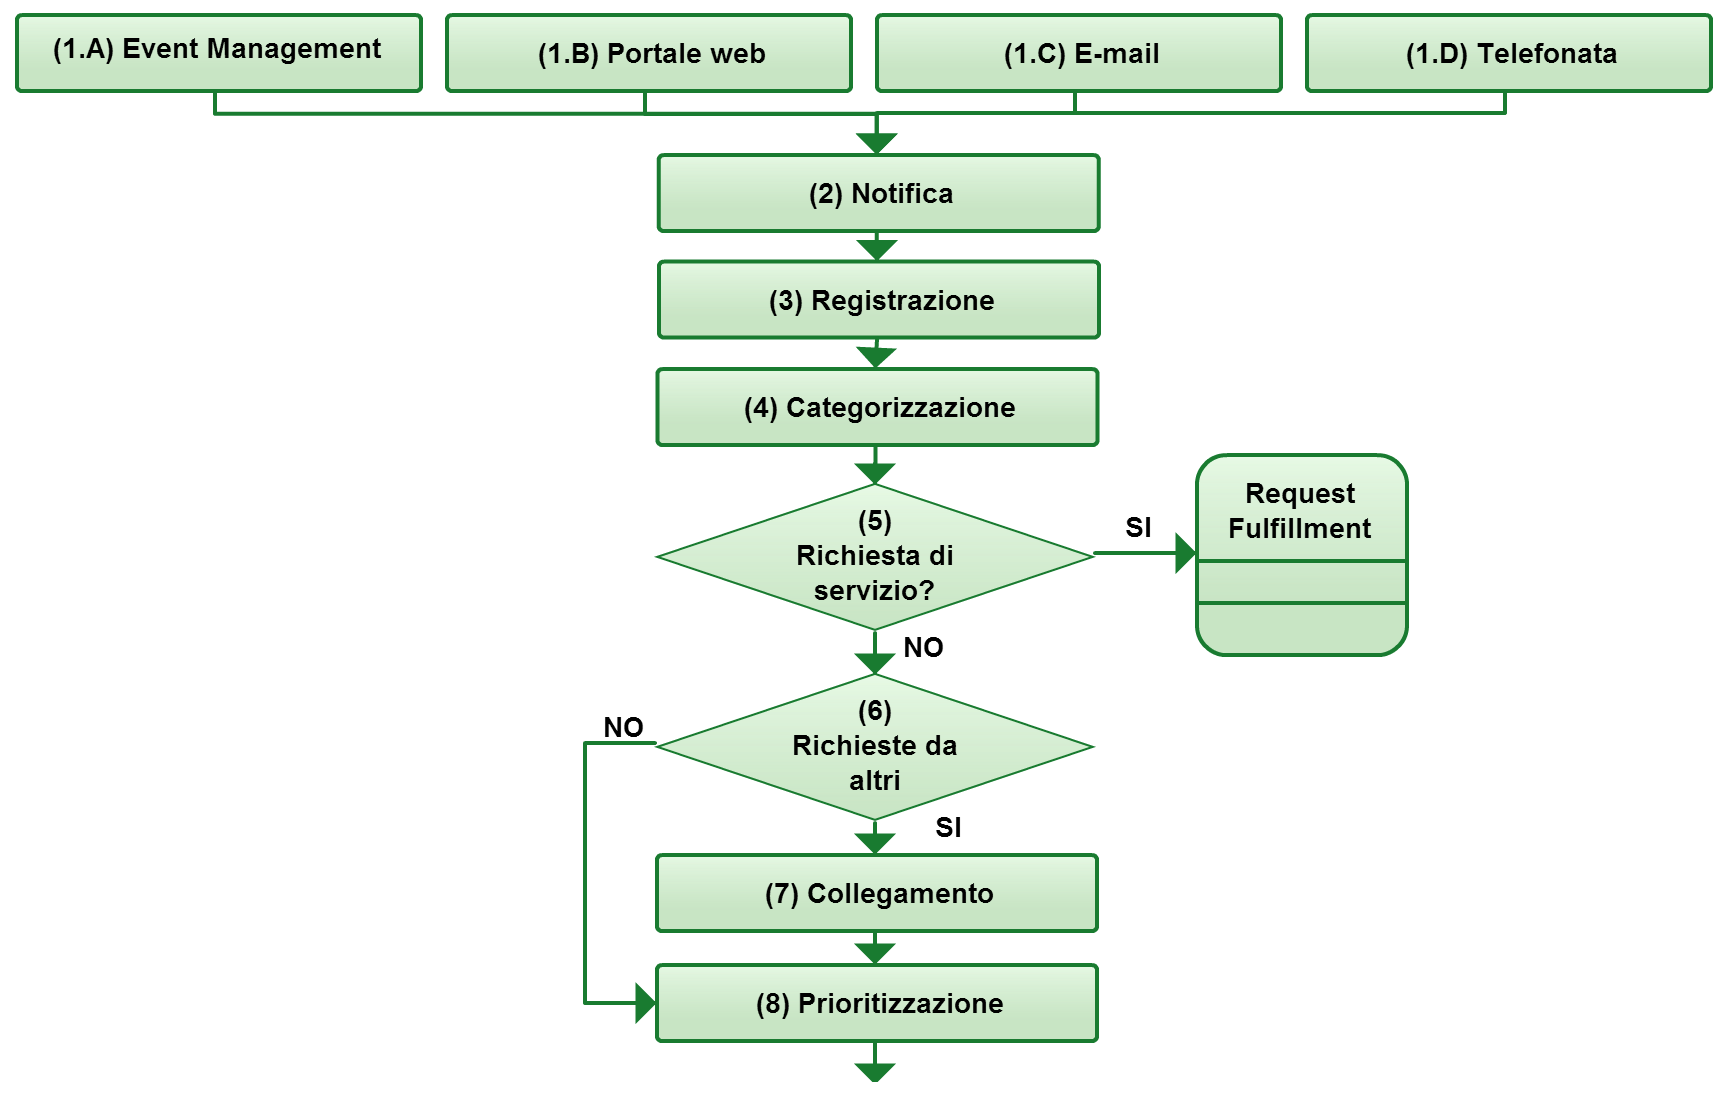
\includegraphics[scale=0.22]{Images/Incident_management_1.png}
\end{figure}
\end{frame}

\begin{frame}{Attività di processo \small{2/2}}
\begin{figure}
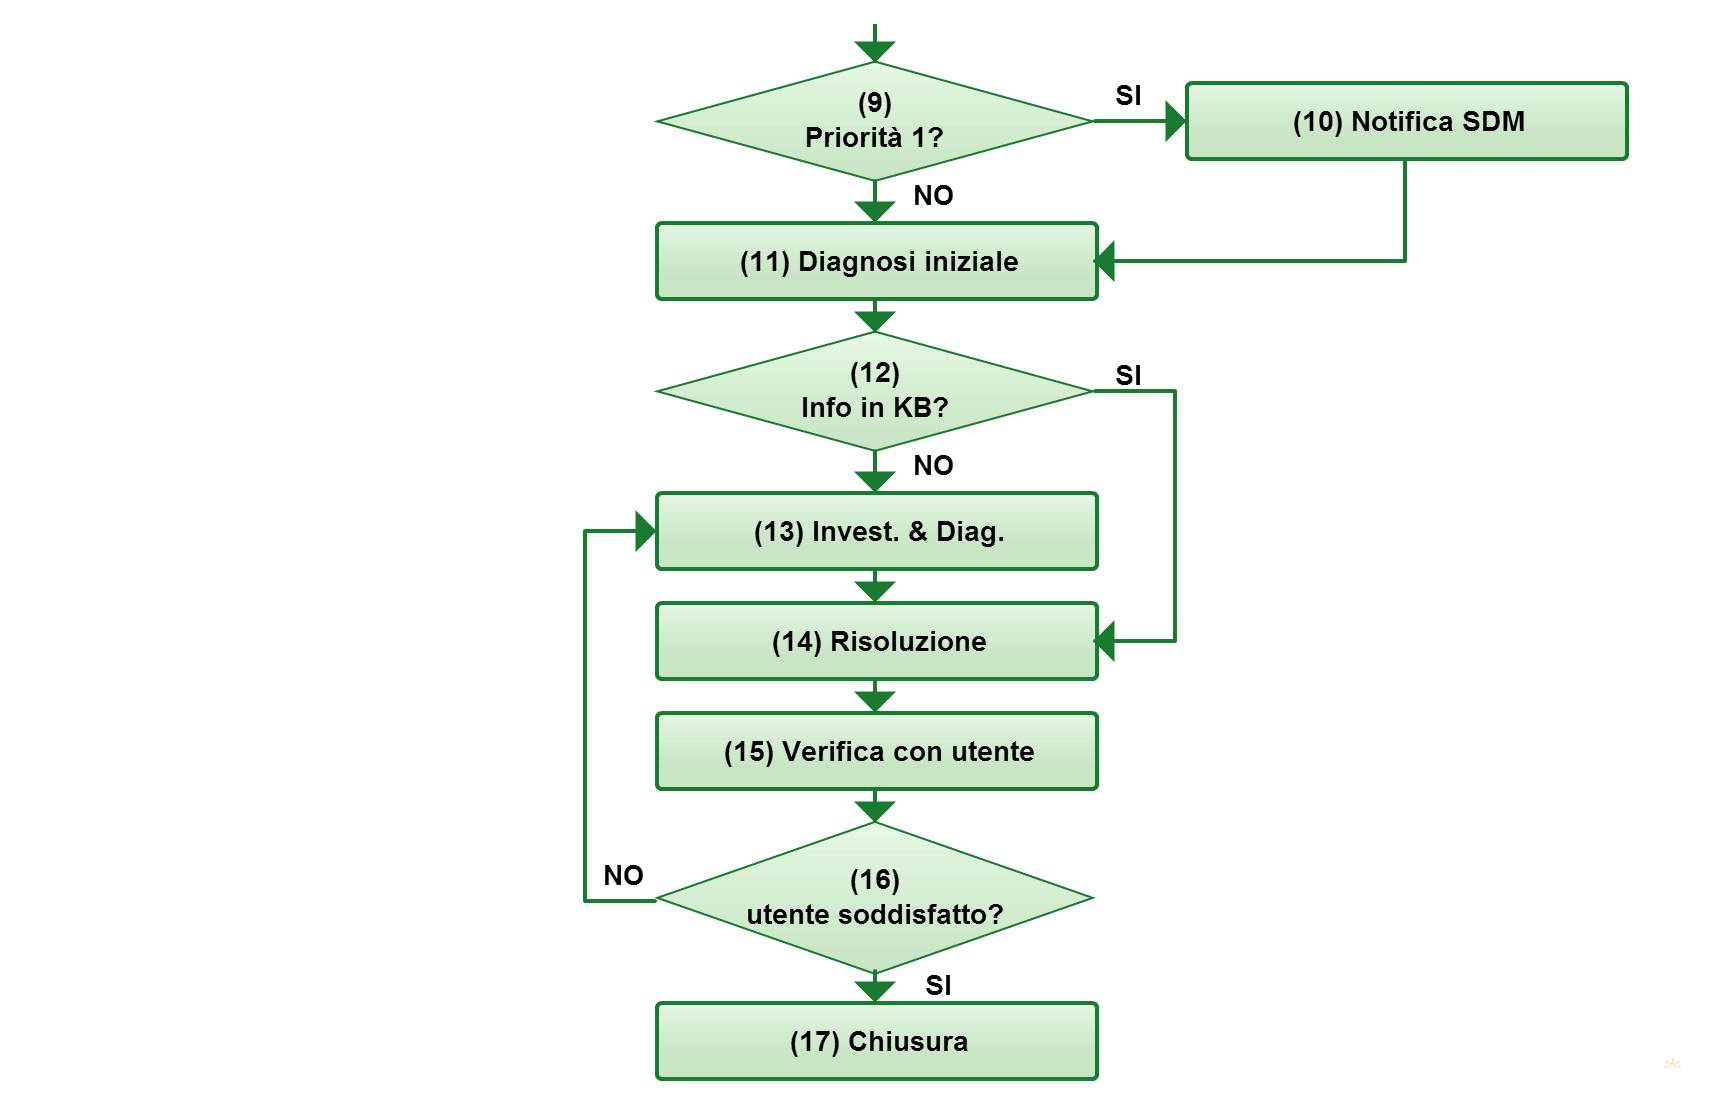
\includegraphics[scale=0.22]{Images/Incident_management_2.png}
\end{figure}
\end{frame}

\subsection*{Attività di escalation}
\begin{frame}{Attività di escalation}
\begin{figure}
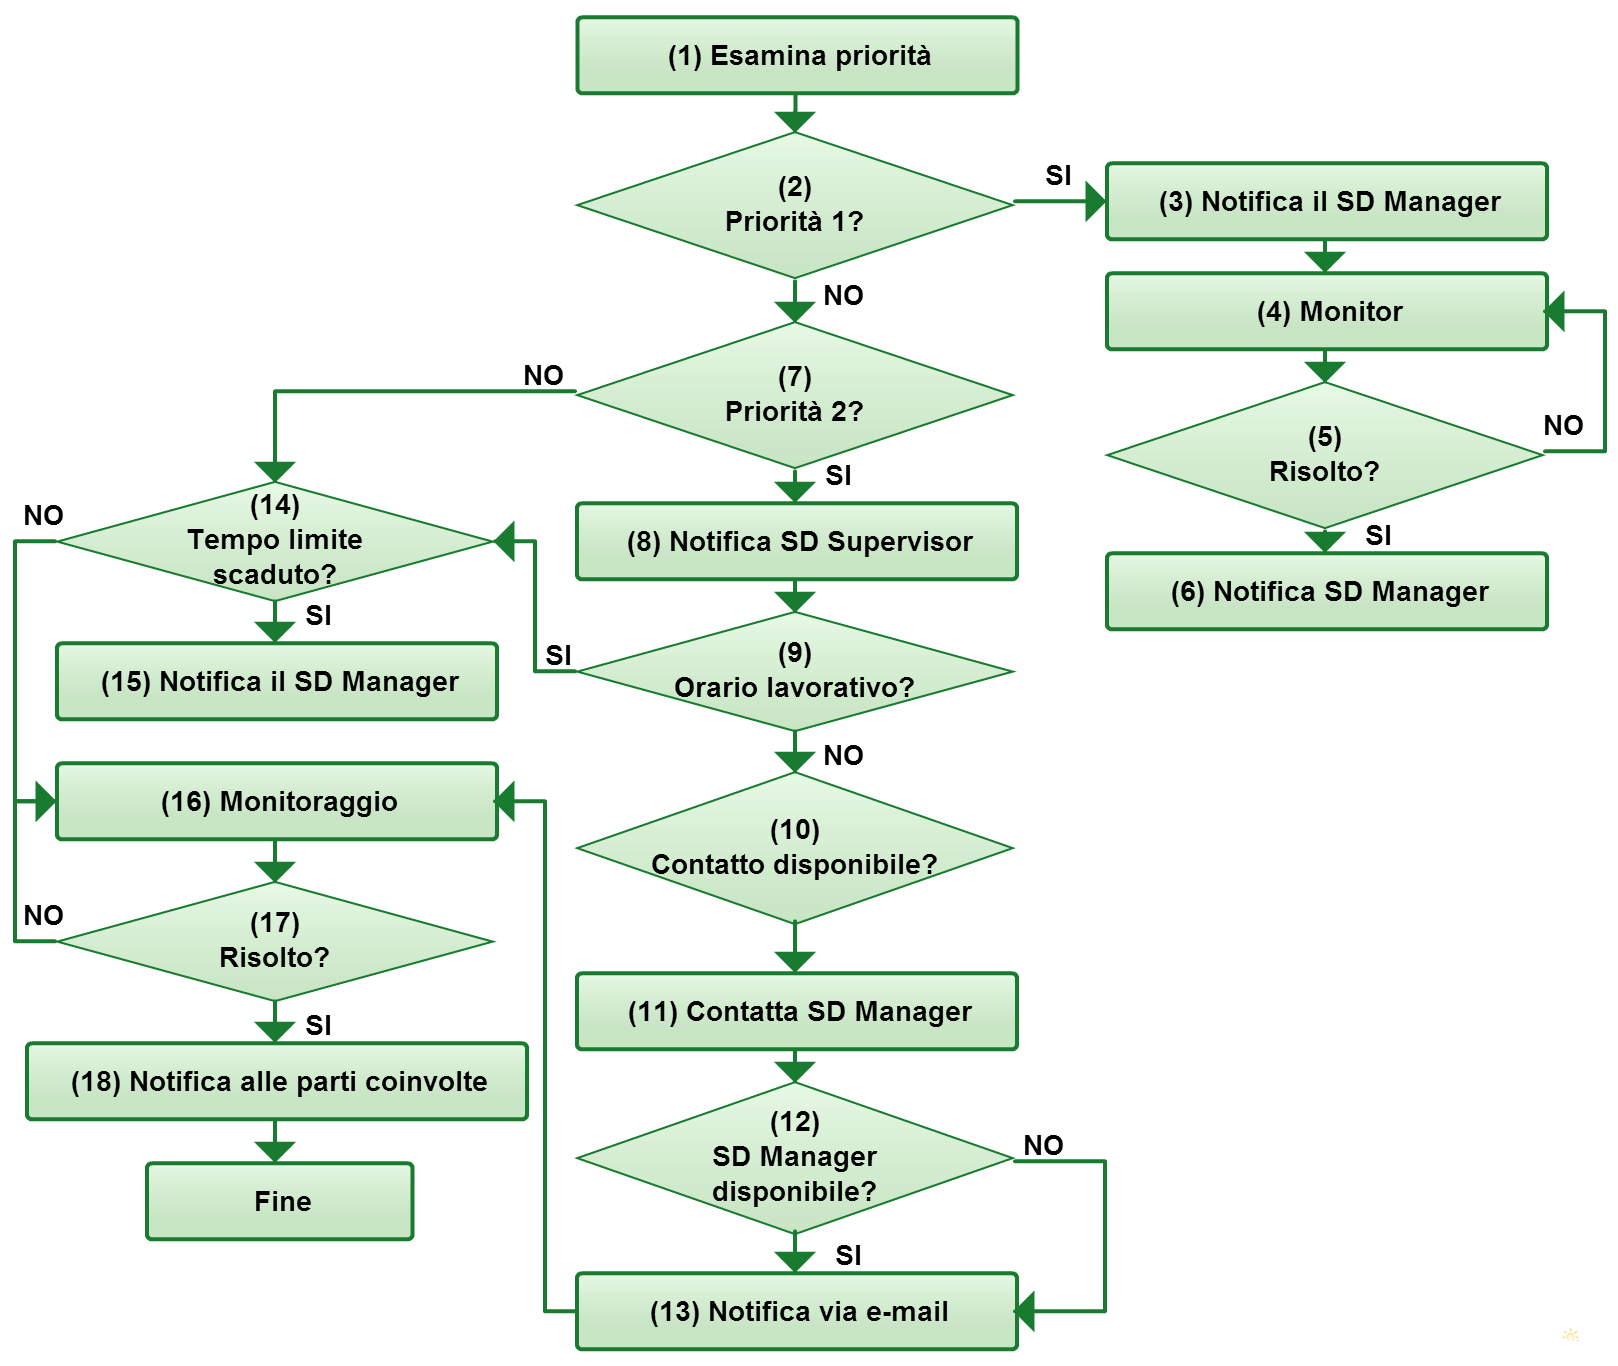
\includegraphics[scale=0.19]{Images/Incident_management_escalation.png}
\end{figure}
\end{frame}